\documentclass[tikz,border=8pt]{standalone}
\usepackage[T1]{fontenc}
\usepackage{amsmath}
\usetikzlibrary{arrows.meta,positioning,fit}

\begin{document}
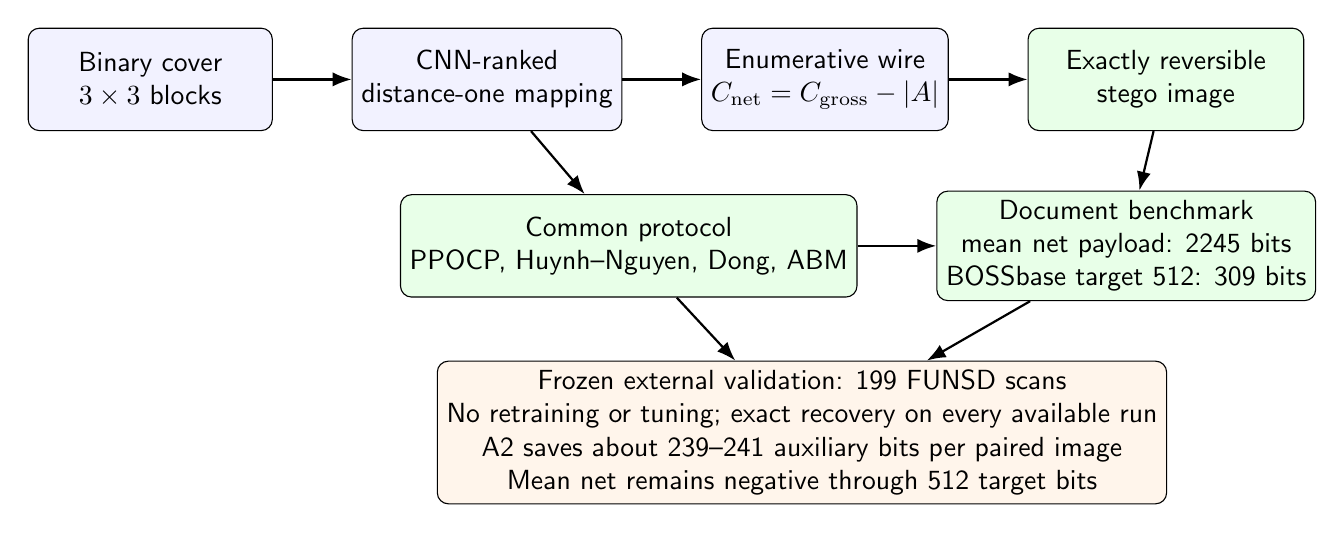
\begin{tikzpicture}[
  font=\sffamily,
  node distance=8mm and 10mm,
  box/.style={draw,rounded corners,align=center,minimum height=13mm,
    minimum width=31mm,fill=blue!5},
  result/.style={draw,rounded corners,align=center,minimum height=13mm,
    minimum width=35mm,fill=green!9},
  evidence/.style={draw,rounded corners,align=center,minimum height=13mm,
    minimum width=49mm,fill=orange!8},
  arrow/.style={-{Latex[length=2.4mm]},thick}
]
\node[box] (cover) {Binary cover\\$3\times3$ blocks};
\node[box,right=of cover] (rank) {CNN-ranked\\distance-one mapping};
\node[box,right=of rank] (net) {Enumerative wire\\$C_{\rm net}=C_{\rm gross}-|A|$};
\node[result,right=of net] (stego) {Exactly reversible\\stego image};

\node[result,below=of rank,xshift=18mm] (benchmark)
{Common protocol\\PPOCP, Huynh--Nguyen, Dong, ABM};
\node[result,right=of benchmark] (outcome)
{Document benchmark\\mean net payload: 2245 bits\\BOSSbase target 512: 309 bits};

\node[evidence,below=of benchmark,xshift=22mm] (funsd)
{Frozen external validation: 199 FUNSD scans\\No retraining or tuning; exact recovery on every available run\\A2 saves about 239--241 auxiliary bits per paired image\\Mean net remains negative through 512 target bits};

\draw[arrow] (cover) -- (rank);
\draw[arrow] (rank) -- (net);
\draw[arrow] (net) -- (stego);
\draw[arrow] (rank) -- (benchmark);
\draw[arrow] (benchmark) -- (outcome);
\draw[arrow] (stego) -- (outcome);
\draw[arrow] (benchmark) -- (funsd);
\draw[arrow] (outcome) -- (funsd);
\end{tikzpicture}
\end{document}
